% Plantilla de documento para PFG usando memoriaPFC.cls

\documentclass{memoriaPFC}

%% ---------------------------------------------------
%% Datos del resumen y descriptores (para metadatos y resumen)
%% ---------------------------------------------------

\resumen{
  El proyecto tiene como objetivo el diseño y desarrollo de una solución web para la gestión de un equipo deportivo real proporcionando una plataforma eficiente y accesible para los usuarios.

  Esta aplicación permitirá recoger y procesar datos de los partidos de la temporada y estadísticas tanto de jugadores como del equipo. De manera adicional, se encargará de la gestión de las convocatorias y dispondrá de un sistema para anotar las incidencias de los partidos en directo. Se desarrollará un módulo inteligente que, partiendo de la información del equipo y de los jugadores recopilada durante los partidos, podrá realizar recomendaciones de áreas a entrenar. Por último, ofrecerá diversos servicios de apoyo al equipo como un foro de mensajes o la gestión de pedidos de material.

  A la hora de diseñar la solución, se utilizará draw.io para definir su estructura y Figma para el diseño de las pantallas. Para el desarrollo del proyecto, se usarán varias tecnologías como React para la parte frontend y Spring Boot en la parte backend,  Maven, y SQL como base de datos. Se hará uso de Docker para el despliegue de la aplicación.
}

\descriptores{Aplicación web, gestión de equipo deportivo, inteligencia artificial generativa, estadísticas}


%% ---------------------------------------------------
%% Comienzo del documento
%% ---------------------------------------------------

\usepackage{enumitem}
\usepackage{microtype}
\usepackage[table]{xcolor}
\usepackage{array}
\usepackage{booktabs}
\usepackage{colortbl}
\usepackage{xurl}
\usepackage{float}
\usepackage{booktabs}
\usepackage{multirow}
\usepackage{array}
\usepackage{longtable}
\usepackage{graphicx}
\usepackage{needspace}



\begin{document}

%% Selección de idioma del documento
\selectlanguage{spanish}  % Comentar esta línea para redactar en inglés

%% ----------------------
%% Materia preliminar
%% ----------------------

\frontmatter

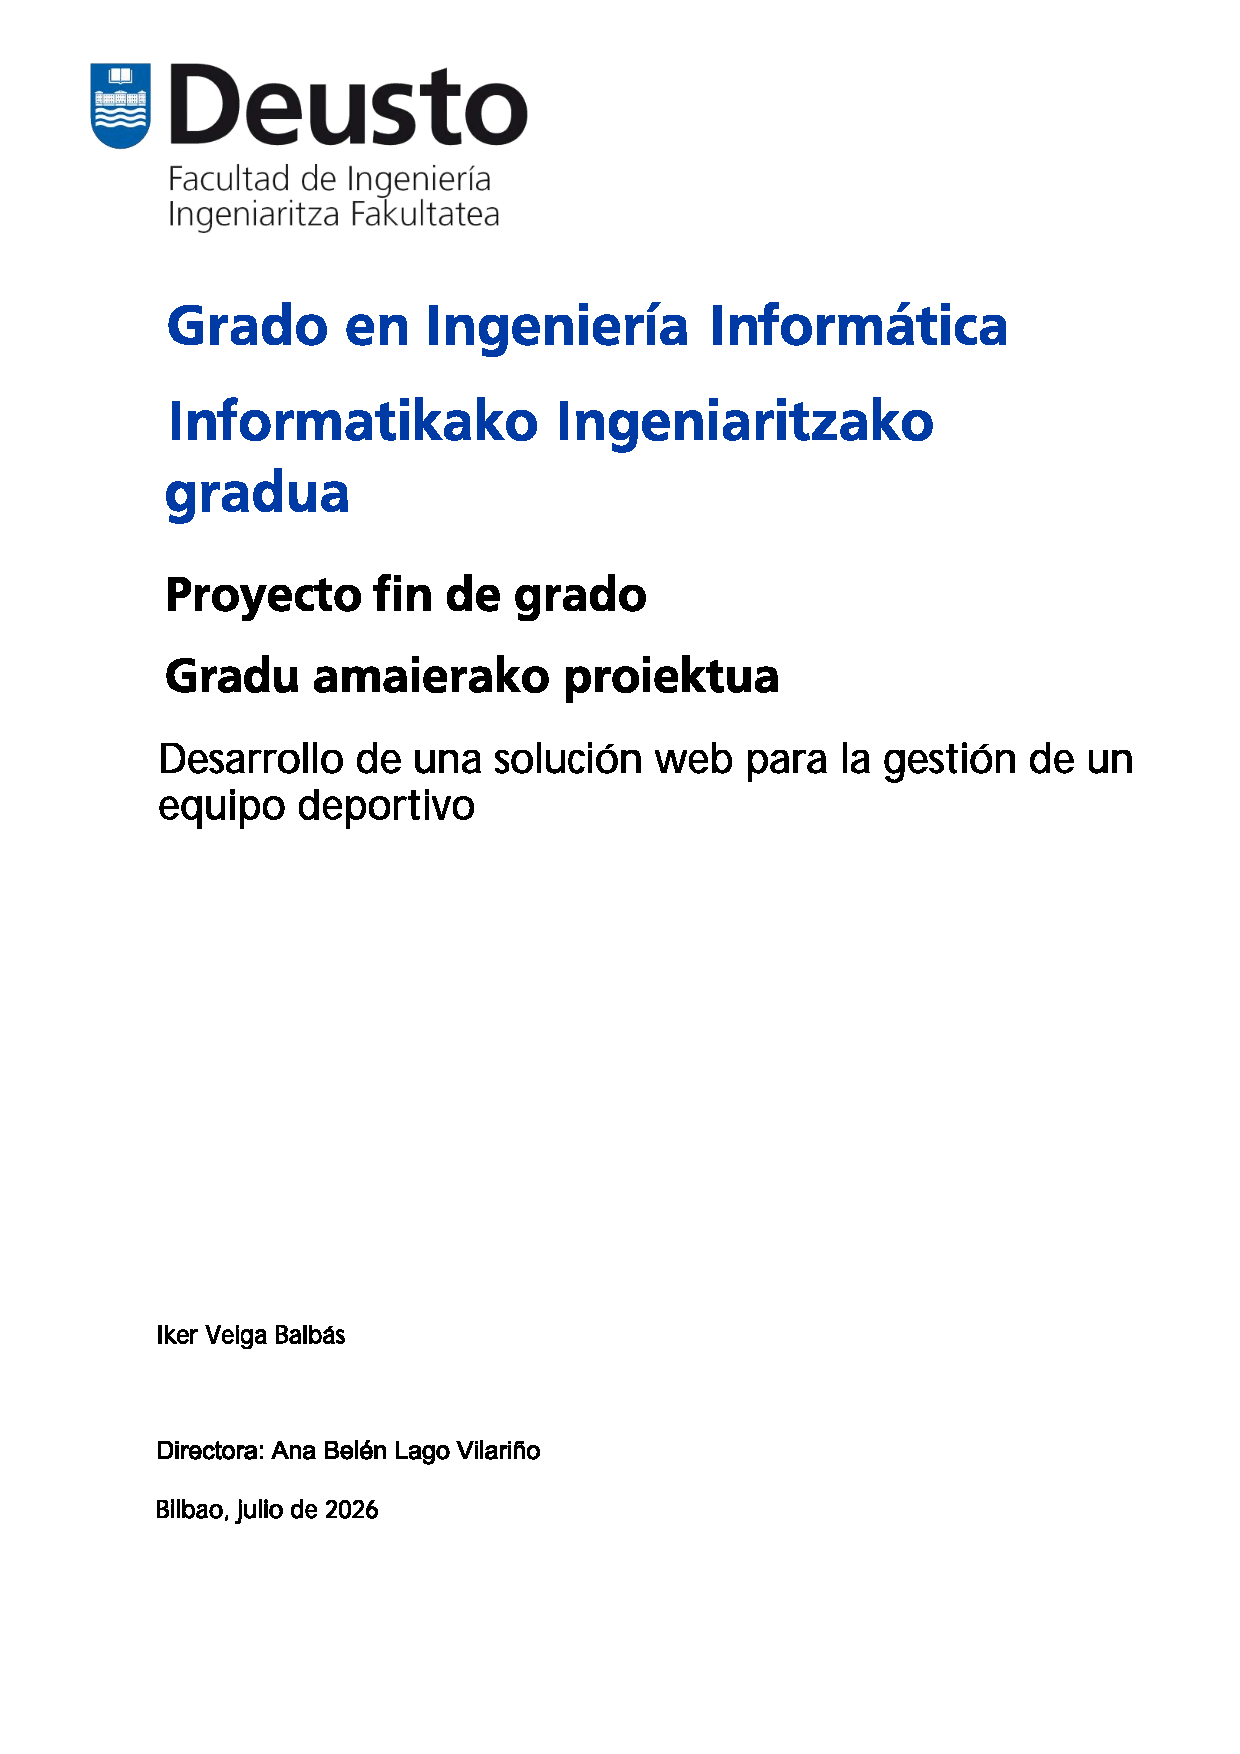
\includepdf[pages=1]{./portada.pdf}          % Portada delantera (opcional)
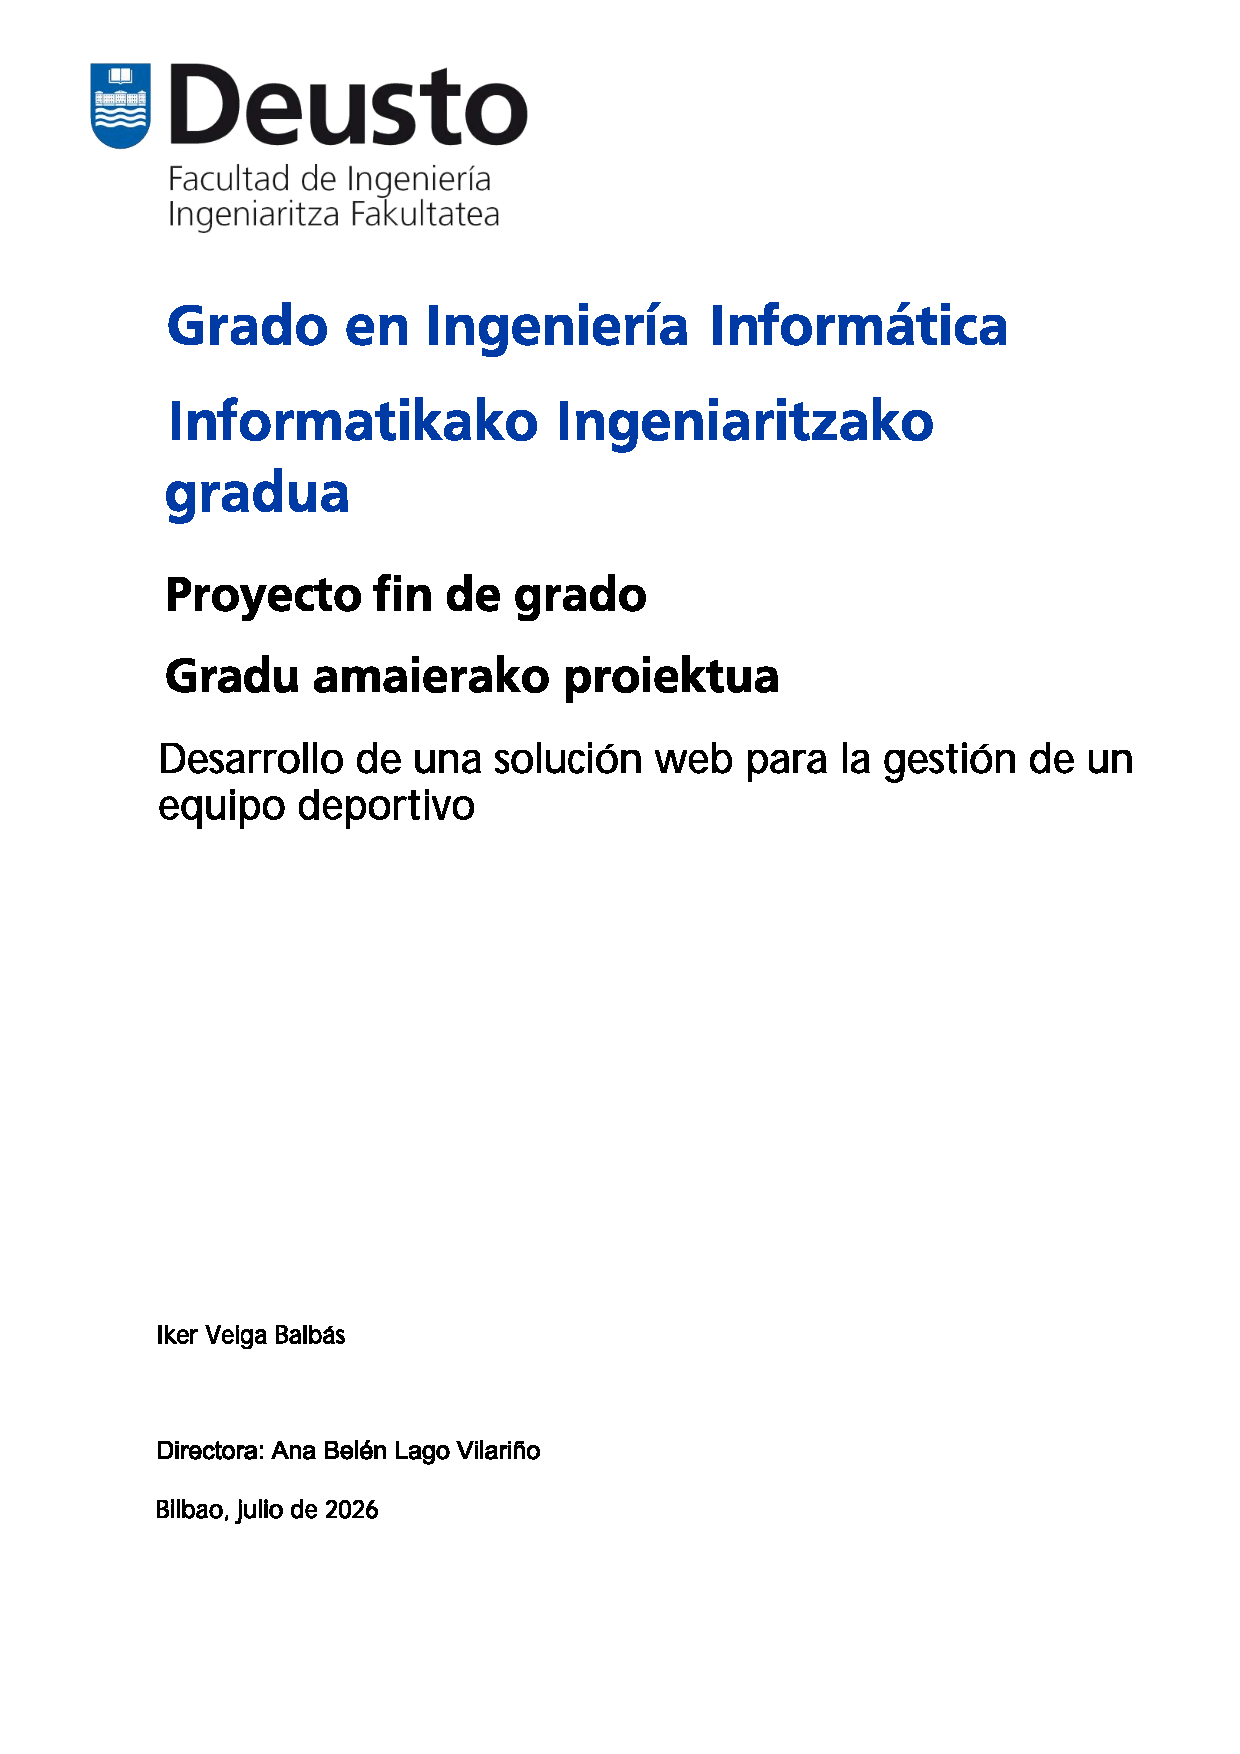
\includepdf[pages=1]{./portada.pdf}  % Portada firmada (opcional)

\resumenPersonalizado{
  El proyecto tiene como objetivo el diseño y desarrollo de una solución web para la gestión de un equipo deportivo real proporcionando una plataforma eficiente y accesible para los usuarios.

  Esta aplicación permitirá recoger y procesar datos de los partidos de la temporada y estadísticas tanto de jugadores como del equipo. De manera adicional, se encargará de la gestión de las convocatorias y dispondrá de un sistema para anotar las incidencias de los partidos en directo. Se desarrollará un módulo inteligente que, partiendo de la información del equipo y de los jugadores recopilada durante los partidos, podrá realizar recomendaciones de áreas a entrenar. Por último, ofrecerá diversos servicios de apoyo al equipo como un foro de mensajes o la gestión de pedidos de material.

  A la hora de diseñar la solución, se utilizará draw.io para definir su estructura y Figma para el diseño de las pantallas. Para el desarrollo del proyecto, se usarán varias tecnologías como React para la parte frontend y Spring Boot en la parte backend,  Maven, y SQL como base de datos. Se hará uso de Docker para el despliegue de la aplicación.
}{Aplicación web, gestión de equipo deportivo, inteligencia artificial generativa, estadísticas}

%% Índices
\tableofcontents
\listoffigures        % Opcional
\listoftables         % Opcional

%% ----------------------
%% Contenido principal
%% ----------------------

\mainmatter

%% Contenido principal (usar \input para incluir capítulos externos)
\chapter{Introducción}

El presente documento trata el trabajo realizado para el desarrollo del Proyecto Fin de Grado. Trabajo en el que he aplicado todas las competencias adquiridas durante los cuatro años que conforman el grado universitario. En esta memoria se recoge con detalle el proceso hasta llegar al resultado final del proyecto, pasando por la idea, el diseño y el desarrollo de la solución web.

Esta memoria está dividida en varios capítulos, con el objetivo de facilitar su lectura y compresión. Dichos capítulos corresponden a los definidos en la especificación de pryectos fin de grado de ingeniería informática proporcionada por la Universidad de Deusto.

\begin{itemize}
  \item Antecedentes y justificación: En este capítulo se recogerá el motivo por el que se ha elegido desarrollar este proyecto. Además, se proporcionarán una serie de antecedentes para entender el pasado de la gestión del equipo deportivo que se ha tomado como referencia, así como su situación actual.
  \item Objetivos y alcance: Es importante fijar el alcance y los objetivos que se desean cumplir con el proyecto. Este capítulo redacta las funcionalidades que recoge el proyecto y los objetivos que se pretenden lograr con la solución web.
  \item Planificación
  \item Presupuesto: Todo proyecto debe tener una estimación del presupuesto, con el fin de aproximar lo máximo posible el coste total que conllevará. En este capítulo se recoge con detalle ese presupuesto, teniendo en cuenta costes de material, costes de desarrollo, costes de puesta en marcha y costes de recurrentes.
  \item Desarrollo del proyecto:
  \item Valoración ética del proyecto
  \item Conclusiones
  \item Bibliografía
  \item Definiciones, acrónimos y abreviaturas
  \item Apéndices
\end{itemize}

\chapter{Antecedentes y justificación}

Vivimos en un país en el que los deportes por excelencia siempre han sido el fútbol y el baloncesto, aunque también hay muchos más deportes con gran visibilidad en España. No obstante, también existen cantidad de deportes minoritarios en nuestro país. Estos deportes carecen de profesionalización debido a la escasa visibilidad que se les proporciona. Por ello, estos clubes disponen de recursos mucho más limitados que los de los clubes deportivos profesionales.

El hockey línea en España es un deporte minoritario y semiprofesional, que en los últimos años ha ganado mucha visibilidad gracias a la retransmisión en directo de sus partidos en YouTube. Lamentablemente, no es suficiente para profesionalizar este deporte.

El club deportivo tomado como referencia gestiona los procesos de sus distintos equipos acorde a su profesionalidad. Esto implica que dichos procesos (convocatorias, avisos, pedidos de material, análisis de partidos, etc.) se lleven a cabo a través del grupo de Whatsapp del equipo, de la Intranet del club o de otra herramienta. Esto hace que sea necesario disponer de varias aplicaciones ditintas, haciendo que la gestión de los equipos sea un proceso engorroso.

Este proyecto surge de la idea de proporcionar una solución web que centralice esos procesos del club deportivo semiprofesional.

\chapter{Objetivos y alcance}

\section{Objetivos}

El objetivo principal de este proyecto es diseñar y desarrollar una solución web que organizace y facilite los procesos de gestión de un equipo deportivo, a la vez que proporciona herramientas para mejorar su rendimiento. Cabe resaltar que este proyecto ha sido diseñado para uno de los equipos de un club en específico. Para lograr el objetivo principal del proyecto, se han establecido varios objetivos basándose en el principal. Estos objetivos servirán para comprobar si el reusltado final del proyecto es un éxito o un fracaso. Dichos objetivos son los siguientes:

\begin{itemize}
  \item Objetivo 1: Diseñar y desarrollar una aplicación web que centralice los procesos de gestión más importantes y repetitivos del equipo deportivo.
  \item Objetivo 2: Implementar un sistema de seguimiento de incidencias y estadísticas de los partidos en directo.
  \item Objetivo 3: Desarrollar un módulo inteligente que ofrecezca recomendaciones sobre aspectos del partido a mejorar.
  \item Objetivo 4: Implementar distintos tipos de roles para el acceso a la aplicación web.
  \item Objetivo 5: Diseñar una interfaz original y personalizada para el club deportivo de referencia.
  \item Objetivo 6: Desarrollar una aplicación web adaptable a cualquier tipo de pantalla y dispositivo.
\end{itemize}

\section{Alcance}

Dado el carácter académico de este trabajo, el proyecto ha sido desarrollado con recursos y tiempo limitados. Esto implica que su alcance ha tenido que determinarse con claridad desde el principio. Además, se planea la ampliación del proyecto una vez realizada su defensa, por lo que delimitar sus funcionalidades para la presentación en la universidad ha sido una parte importante.

\begin{enumerate}
  \item Desarrollo de la base de datos.
  \item Desarrollar el sistema de login.
  \item Desarrollar el sistema de visualización de próximos partidos.
  \item Desarrollo del sistema de visualización de estadísticas.
  \item Desarrollar el sistema de convocatorias para los próximos partidos.
  \item Desarrollo de la API REST.
  \item Implementación del modelo de Inteligencia Artificial generativa.
  \item Desarrollar el sistema de seguimiento de partidos en directo.
\end{enumerate}

\chapter{Planificación}

\chapter{Presupuesto}

\chapter{Desarrollo del proyecto}

\chapter{Valoración ética del proyecto}

\chapter{Conclusiones}

\chapter{Definiciones, acrónimos y abreviaturas}

\chapter{Apéndices}




%% ----------------------
%% Bibliografía y apéndices
%% ----------------------

\backmatter
\nocite{*}
\bibliografia{referencias}  % Archivo BibTeX: referencias.bib

\appendix
\chapter{Uso de inteligencia artificial}

El objetivo de este anexo es declarar de manera transparente el uso que se ha hecho de la inteligencia artificial en este proyecto.

Este proyecto fue elaborado con la ayuda de varias inteligencias artificiales generativas distintas. En concreto ChatGPT, Claude y Gemini.

Las herramientas previamente mencionadas fueron utilizadas, en primer lugar, como fuente de información. Estas inteligencias artificiales son capaces de contestar casi cualquier pregunta que se les haga. Entonces, aproveché esa característica para intentar resolver dudas o buscar información sobre aspectos que no conocía a la hora de desarrollar el proyecto. Para ello, las inteligencias artificales más utilizadas fueron ChatGPT y Claude.

En segundo lugar, se hizo uso de este tipo herramientas para ayudar a localizar errores en el código más rápidamente. Normalmente las funcionalidades que se implementan no funcionan correctamente a la primera y aparece algún error en la consola. Gracias a que Antigravity IDE integra herramientas de IA para apoyar al desarrollador, aproveché el chat que trae consigo. Cuando aparecía un error en la consola o una funcionalidad no funcionaba como debería, se hacía uso de ese chat para preguntar qué era lo que pasaba y de dónde provenía el error, con el propósito de ahorrar tiempo. Una vez el error era localizado y comprendida su aparición gracias a la respuesta del chat, era resuelto por cuenta propia. Para ello, las inteligencias artificiales más utilizadas fueron Gemini y Claude.

Finalmente, este documento ha sido realizado con apoyo de herramientas de inteligencia artificial con el propósito de corregir errores ortográficos que se han podido pasar por alto.

Cabe destacar que una vez recibidas las respuestas por parte de cualquiera de las inteligencias artificiales utilizadas en este proyecto, éstas eran posteriormente interpretadas, evaluadas y revisadas por el equipo humano que ha relizado el proyecto, con el fin de garantizar la precisión, consistencia, falta de sesgos y veracidad de las mismas.

\end{document}
